\chapter{Functions and sensor options}
IV-Evo uses selectable applications for the display and sensor scripts for measurement. Configure it over Wi-Fi from a phone or computer. Lua scripts allow custom applications and sensor calibration. Select a sensor script and calibration that match the installed hardware.

Available applications include:
\begin{itemize}
\item IV-Evo  Barometer
\item IV-Evo Thermo
\item IV-Evo Voltmeter
\item IV-Evo Gear indicator
\item IV-Evo Lambda
\item IV-Evo Boost
\item IV-Evo Clock
\end{itemize}
The Check Engine application is also described in this manual.

IV-Evo  Barometer is intended to be working with VAG pressure sensor p.No 03C906051A

IV-Evo Thermo is intended to be working with temperature sensor Ossca 01176 or compatible for Golf 2.

\begin{figure}[htbp]
\centering
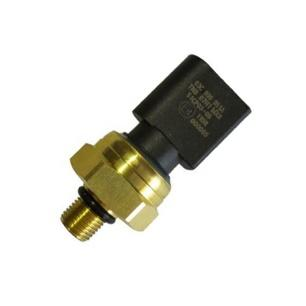
\includegraphics[width=.85\textwidth,height=.60\textheight,keepaspectratio]{figures/ivevo/image21.jpg}
\caption{Sensor reference}
\end{figure}
\begin{figure}[htbp]
\centering
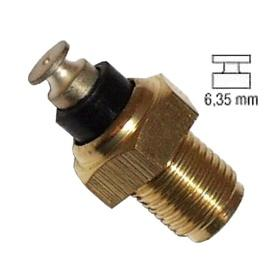
\includegraphics[width=.85\textwidth,height=.60\textheight,keepaspectratio]{figures/ivevo/image19.jpg}
\caption{Sensor reference}
\end{figure}
